\chapter{Evaluation of MELON}\label{chapter:evaluation}

\section{Performance Analysis}

\subsection{Operation Speed}

\begin{figure}
\centering
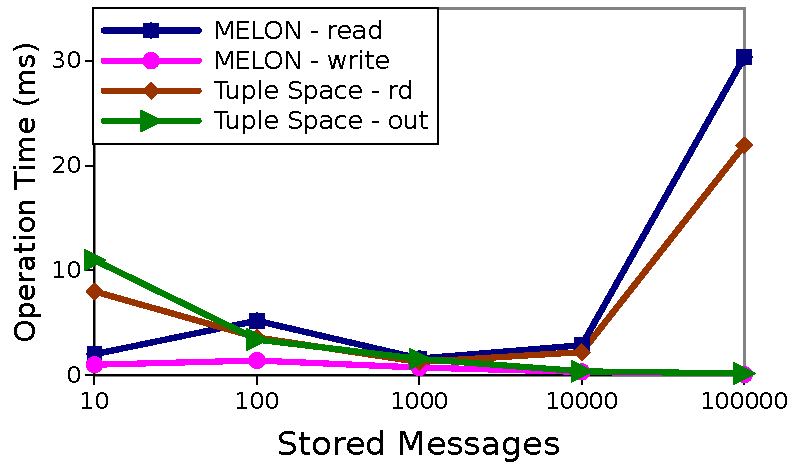
\includegraphics[width = \linewidth, clip, trim = 0px 0px 0px 0px]{figures/read_speed.pdf}
\caption{Read Speed}
\label{fig:readspeed}
\end{figure}

\begin{figure}
\centering
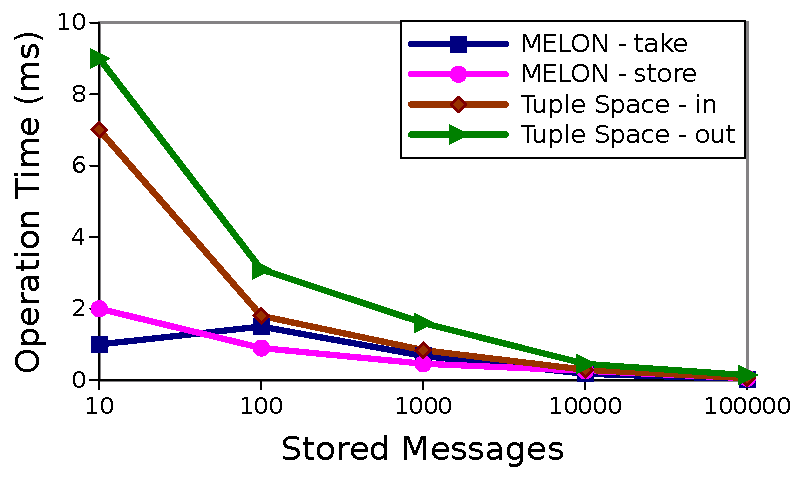
\includegraphics[width = \linewidth, clip, trim = 0px 0px 0px 0px]{figures/in_speed.pdf}
\caption{Take Speed}
\label{fig:takespeed}
\end{figure}

To establish a baseline for performance, we measured the time for the \textbf{write}, \textbf{read}, \textbf{store}, and \textbf{take} operations directly on a local message storage and compared the results to the LighTS\cite{lights} local tuple space implementation used by LIME. In these experiments, all messages are first stored, then either read or removed from the local storage. No network communication is involved.

When comparing \textbf{read} and \textbf{rd}, we simulate the MELON's feature of only returning unread messages by using a sequential integer ID in the tuples and performing a \textbf{rd} operation for each ID. If we did not do this, LighTS would return the same tuple for each \textbf{rd} operation.

In both LighTS and MELON, messages are stored in what is essentially an array. Since we are not removing messages, each operation must linearly search the array taking O(\textit{nm}) time, where \textit{n} is the length of the message or tuple and \textit{m} is the number of stored messages or tuples. Naturally, operations returning messages near the beginning of the array are faster, while the slowest operation returns the last message in the array. In our experiments, this cost did not become apparent until searching 100,000 messages. The average time per operation from 10,000 to 100,000 increased \~9x for LighTS and \~10x for MELON, with total read time taking just under a minute. It is unsurprising MELON is slightly slower, since it must also check that a message is not in the ``read'' list before returning it.

On the other hand, removing messages is naturally quite fast, since the matching message is always the first message in the store. All \textbf{take}/\textbf{in} operations require less than 8\textit{ms} to execute on average. MELON is slightly faster here due to differences in how removal is implemented, although average speed per operation converges as the number of operations performed increases.

Storing messages is faster than removing them for both implementations. In LighTS there is slightly more constant overhead for adding new tuples, so \textbf{out} operations are a little slower than \textbf{write} and \textbf{store} in MELON.  However, in reality both implementations are plenty fast for typical applications, since storing a message takes less than 10\textit{ms} on average, and usually less than 4\textit{ms}.

Overall, MELON performs roughly the same or better than LighTS when performing serial operations.

\subsection{Communication Overhead}

\begin{figure}
\centering
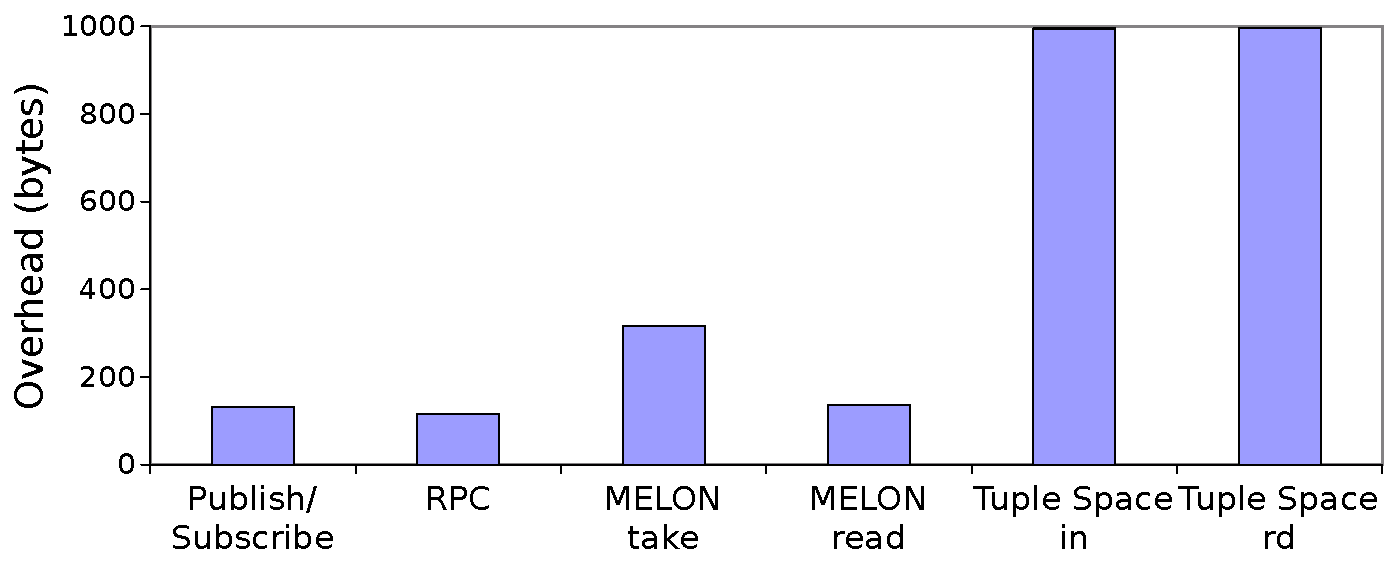
\includegraphics[scale = .50, clip, trim = 0px 0px 0px 0px]{figures/overhead.pdf}
\caption{Message Overhead}
\label{fig:overhead}
\end{figure}

For any communication library or framework, the message size added by use of the library is an important factor in determining its usefulness. In these experiments, we measure the number of bytes actually sent over the network, divide by the number of messages sent (in this case, 1000) and subtract the 1KB application payload. This leaves us with the overhead introduced by the paradigm. We compare the overhead of MELON to canonical implementations of publish/subscribe, RPC, and tuple spaces in Figure \ref{fig:overhead}.

Publish/subscribe and RPC have very low overhead and provide a good baseline. In the case of publish/subscribe, the only added information to a publication is the topic. Periodic subscription messages are small and infrequent compared to the number of messages sent. For RPC, there is one initial exchange to find the remote object, then later messages only need the object and method names plus the payload itself.

As in the operation speed experiments, we use the LighTS tuple space implementation. The serialized versions of tuples and tuple templates are very large and must be sent for each request. If a simpler data structure were used, overhead would be expected to be similar to MELON's overhead for \textbf{take}.

For MELON, \textbf{take} and \textbf{read} requests must send a message template, so the size of the request is dependent on how many values the template contains. For \textbf{read} operations, each request must also send information on previously read messages as described in Section \ref{sec:readmessages}, which increases as the number of read messages increases.

\subsection{Message Latency}

\begin{figure}
\centering
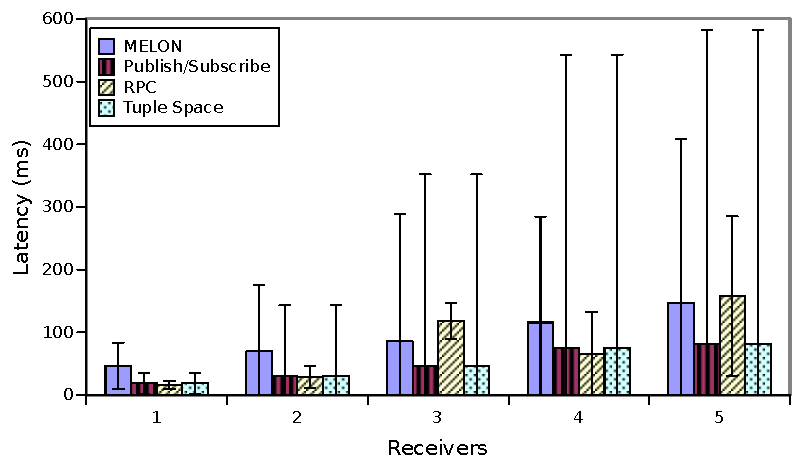
\includegraphics[width = \linewidth, clip, trim = 0px 0px 0px 0px]{figures/latency_static.pdf}
\caption{Message Latency - Static Scenario}
\label{fig:latencystatic}
\end{figure}

\begin{figure}
\centering
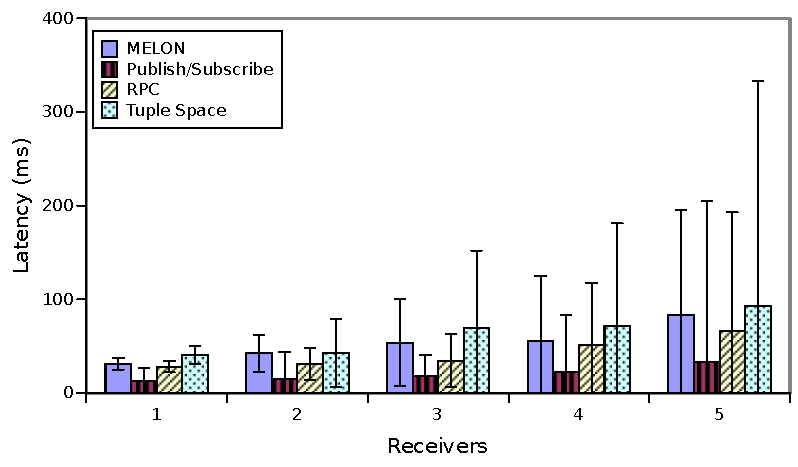
\includegraphics[width = \linewidth, clip, trim = 0px 0px 0px 0px]{figures/latency_mobile.pdf}
\caption{Message Latency - Mobile Scenario}
\label{fig:latencymobile}
\end{figure}

Figures \ref{fig:latencystatic} and \ref{fig:latencymobile} show the average latency between a client's request for a message and the receipt of a matching message. The error lines indicate the standard deviation. In these experiments, a single host writes out 1,000 messages with a 1KB payload, and the other hosts concurrently read the messages. Tuple spaces and MELON used the \textbf{rd}/\textbf{read} operations to retrieve the messages one at a time, rather than the bulk retrieval with \textbf{rdg} or \textbf{read\_all}. Since publish/subscribe does not involve a ``request'' beyond the initial operation, latency was measured as the time elapsed between receiving sequentially numbered publications.

MELON does show higher average latency rates in the static scenario, although for three or more receivers the standard deviation is lower than the other paradigms. In the more realistic mobile scenario, however, MELON latency is about the same or slightly lower than tuple spaces. Comparing the static and mobile scenarios also demonstrates one of the issues in wireless networks: the mobile scenario allows distinct routes to form between hosts with less interference, while the static scenario has many collisions causing more communication delays even though the distance between devices is smaller.

\subsection{Message Throughput}

\begin{figure}
\centering
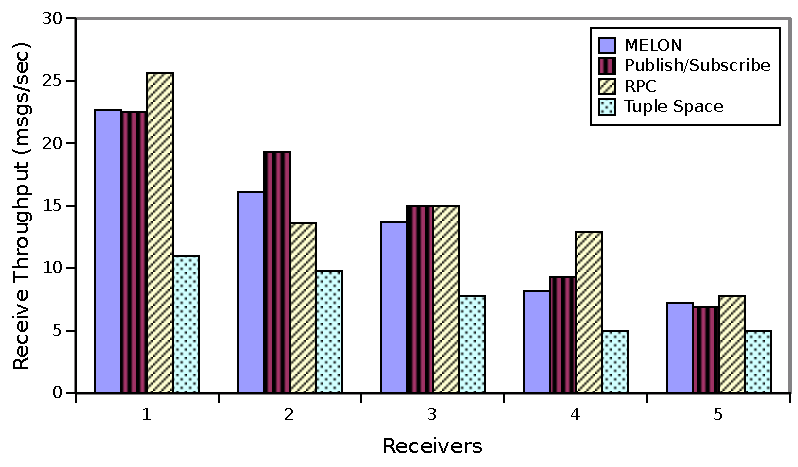
\includegraphics[width = \linewidth, clip, trim = 0px 0px 0px 0px]{figures/throughput_static.pdf}
\caption{Message Throughput - Static Scenario}
\label{fig:throughputstatic}
\end{figure}

\begin{figure}
\centering
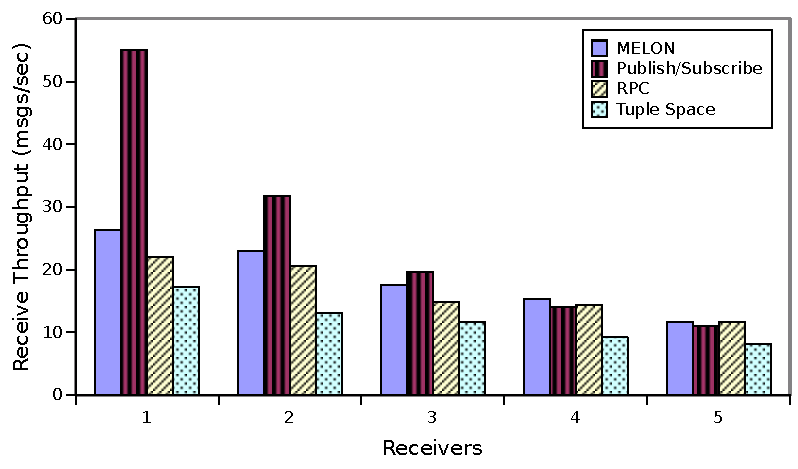
\includegraphics[width = \linewidth, clip, trim = 0px 0px 0px 0px]{figures/throughput_mobile.pdf}
\caption{Message Throughput - Mobile Scenario}
\label{fig:throughputmobile}
\end{figure}

Throughput in these experiments was measured on the receiver side in terms of messages delivered per second. As in the other experiments, 1,000 messages with a 1kb payload are output by one host, while the other hosts read the messages one at a time. Figures \ref{fig:throughputstatic} and \ref{fig:throughputmobile} show the average throughput as the number of receivers increases.

Publish/subscribe dominates in these experiments since it is the only push-based paradigm, allowing the sender to publish messages at a high rate without requests or acknowledgments from the receivers. Also, subscribers may receive multiple publications concurrently which increases throughput capacity.

Despite having higher average latency than the other paradigms, MELON demonstrates good throughput in both the static and mobile scenarios. However, throughput for all paradigms drops off dramatically as more receivers are added. Also, all paradigms performed better in the mobile scenario than in the static scenario. This is likely due to two factors: devices were not forced to be more than one hop apart, and the large number of devices allows distinct routes between devices and decreases wireless broadcast collisions.


\subsection{Whiteboard Performance}

For each implementation, we measured the number of messages lost, the number of messages received out of order, and the message latency. For out-of-order messages, we divided it into two metrics: host out-of-order and global out-of-order. Host out-of-order messages are messages from a single host which are not received in the order sent. Global out-of-order messages are those received before their preceding message. For example, if node A receives a message \textit{m}$_{1}$ from node B, then sends \textit{m}$_{2}$. If node C receives \textit{m}$_{2}$ prior to \textit{m}$_{1}$, \textit{m}$_{2}$ will be considered out of order.

\begin{figure}[ht]
\centering
\begin{minipage}[b]{0.48\linewidth}
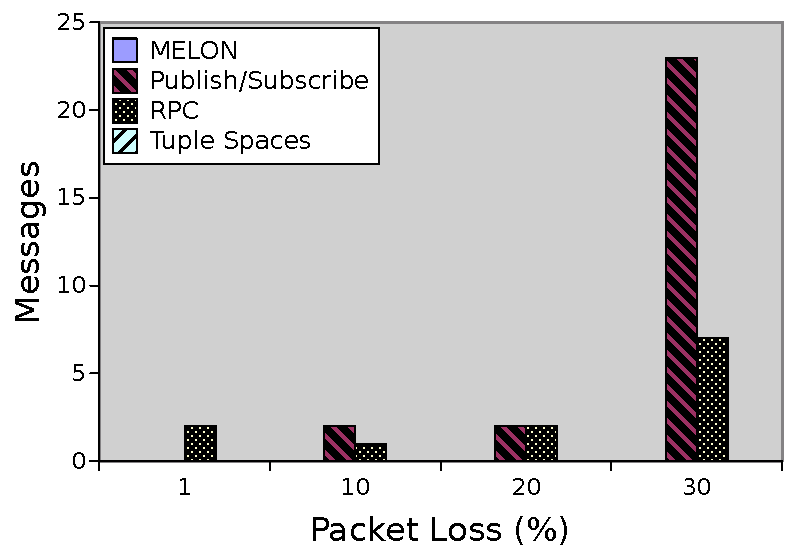
\includegraphics[width = \textwidth]{figures/hooo.pdf}
\caption{Host Out-of-Order Messages}
\label{fig:hooo}
\end{minipage}
\quad
\begin{minipage}[b]{0.48\linewidth}

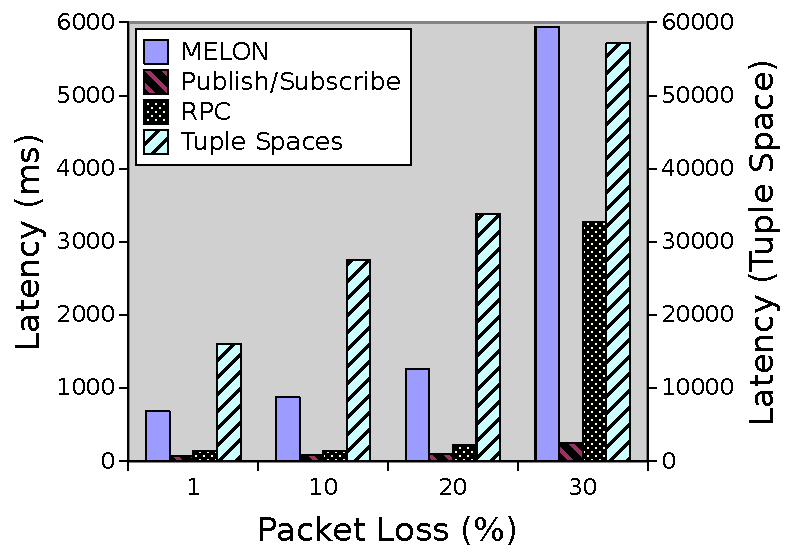
\includegraphics[width = \textwidth]{figures/latency.pdf}
\caption{Message Latency}
\label{fig:latency}
\end{minipage}
\end{figure}
\begin{figure}[ht]
\centering
\begin{minipage}[b]{0.48\linewidth}
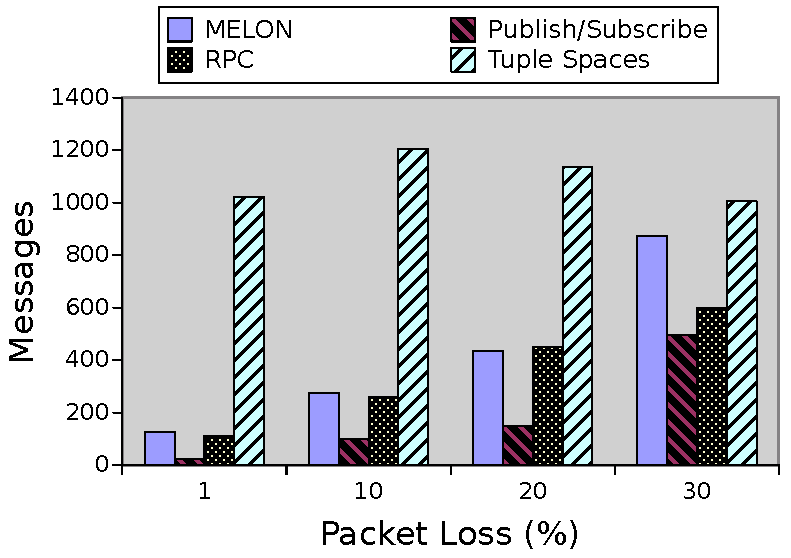
\includegraphics[width = \textwidth]{figures/gooo.pdf}
\caption{Global Out-of-Order Messages}
\label{fig:gooo}
\end{minipage}
\quad
\begin{minipage}[b]{0.48\linewidth}
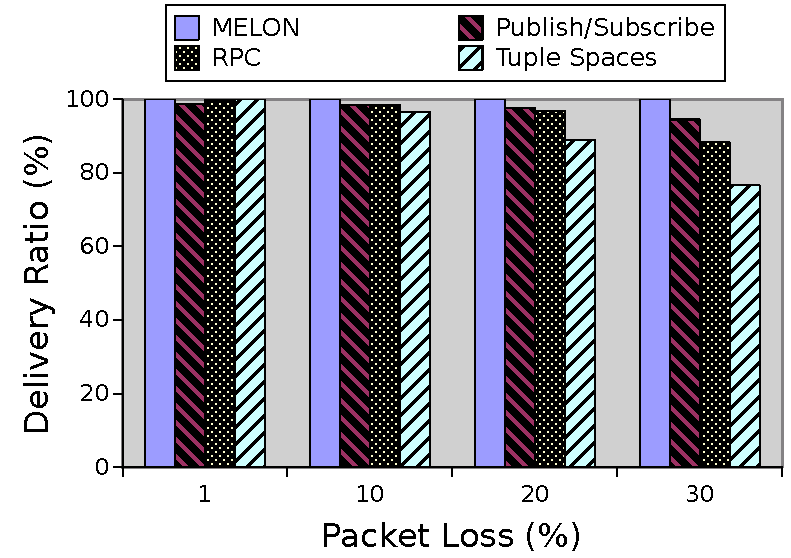
\includegraphics[width = \textwidth]{figures/delivery.pdf}
\caption{Delivery Rates}
\label{fig:delivery}
\end{minipage}
\end{figure}

In our experiments, messages from a single host were generally delivered in the order they were sent as shown in Figure \ref{fig:hooo}. For MELON and tuple spaces, no messages were delivered out of order. However, it should be noted that for tuple spaces this is an accident of the implementation, whereas in MELON it is guaranteed. In LighTS, tuples are sequentially stored locally in an array in the order they are output, then returned in that same order when they are matched. Tuple spaces in general do not return matched messages in any particular order.

In this application, RPC is used in an asynchronous manner since it is providing group communication. If one call is delayed, it is possible a subsequent call will complete before a prior one, which explains why RPC delivers a small number of messages out of order. Publish/subscribe is fully asynchronous and incoming publications can even be processed concurrently. However, even in the worst case publish/subscribe delivers 97.8\% of the messages from a host in the order they were sent. Unfortunately, like tuple spaces this is just the result of a single implementation and the RPC and publish/subscribe paradigms make no promises about the ordering of messages.

Unlike per-host ordering, many messages were delivered out of order from a global perspective as can be seen in Figure \ref{fig:gooo}. This is entirely expected, since none of the paradigms provide a global ordering. Enforcing a global ordering in an unreliable network is not feasible, since nodes may become unavailable at anytime while continuing to output messages. However, the global ordering remains important for a shared whiteboard.

Our results show publish/subscribe performs the best for this metric. Indeed, ordering is largely dependent on deliveries completing quickly before later messages overtake them. As shown in Figure \ref{fig:latency}, publish/subscribe is an extremely quick method for delivering messages, so it excels in ordering as well. Conversely, tuple spaces fare the worst, delivering 67\% of messages out of order. Again, because tuple spaces provide no way of controlling which matches messages are returned or in what order, the whiteboard implementation must transfer large amounts of tuples in order to nondestructively read all matching messages. This is extremely slow, as reflected in Figure \ref{fig:latency}.

MELON and RPC perform about the same for global ordering, although MELON is more affected when the network conditions worsen. This is likely due to MELON's reliable message delivery (Figure \ref{fig:delivery}), since some messages may be delayed significantly by broken network routes or network partitioning. In contrast, losing messages can improve ordering since a message not delivered cannot be out of order. Of the paradigms compared, MELON is the only one to demonstrate 100\% message delivery. Tuple spaces would also be expected to be reliable, but again in this application it is required to deliver large amounts of messages. Given that the median latency for tuple spaces reached a full minute, the experiment completed before some messages arrived.

While we have seen publish/subscribe have low delivery ratios in the past\cite{collins2010quantitative}, here it performs well in the lossy environment due to its quick delivery rates, but still dropped 1.4\% of messages when the network connectivity was good. RPC performs predictably, slowing losing more messages as the network degrades. Again, we are using group RPC, which means the application is not aware of how many receivers may be available and therefore does not retry to complete calls if a host cannot be reached for a period of time. Fully synchronous RPC would block the process until the message is delivered. However, that would also delay deliveries considerably which is not acceptable for a whiteboard application.

Median time between sending and receiving a message is reported in Figure \ref{fig:latency}. Since tuple spaces are so much slower, the results are aligned with the right-hand y-axis which is an order of magnitude higher. Publish/subscribe was extremely quick, which is expected since it requires no message confirmations nor active discovery of remote hosts. RPC was also quite fast until it was slowed down along with the other paradigms by the 30\% packet loss.

Logically, delivery rates and latency are directly related. With reliable delivery some messages may be very late, increasing overall latency. On the other hand, dropped messages do not count towards the latency metric, so a lossy communication paradigm can appear to be very fast. MELON errs on the side of reliability, and therefore is a bit slower as the network becomes less reliable and more delivery attempts are required. There is an additional trade-off that pull-based paradigms like MELON and tuple spaces must make, which is the frequency of the pull attempts. Publish/subscribe and RPC may send as soon as a message is ready, but MELON and tuple spaces must continually poll to receive messages. Faster polling results in faster message delivery, but higher overall network usage, collisions and resource monopolization.

\section{MELON Suitability for MANET Applications}

In the previous chapters, we have noted three important features which we believe should be provided by a general purpose communication paradigm for applications operating in a mobile ad-hoc network: \textit{disconnection handling}, \textit{resource addressing and discovery}, and \textit{flexible communication}. This section examines how well MELON implements these features.

\subsection{Disconnection Handling}

MELON does not have a concept of connections exposed to the application layer. Applications are not affected by disrupted or lost connections, because MELON effectively hides these disconnections in its operations. Since MELON provides spatial decoupling, not only does the application not maintain connections to specific hosts, it is completely unaware of the location of any resources to begin with.

Besides intermittent disconnections which may disrupt communications but from which applications can quickly recover, prolonged disconnections where a node is unreachable for some time (but eventually returns) are also common. The message persistence in MELON provides temporal decoupling between nodes, so that a process on one node may output a message which may be read at any later time, possibly much later. This approach adapts well to the MANET environment, where the network topology may be constantly changing. It allows messages to be received opportunistically instead of only having a chance of receiving the message at the time of sending.

Finally, it is possible to provide some message replication in MELON as discussed in Section \ref{sec:replication} in order to deal with permanent disconnections between nodes. Message replication allows messages to potentially cross network partitions by copying messages to nodes which may then travel to parts of the network unreachable by the original sender. It also increases availability of messages and can improve performance if a cached message is available at a node closer than the original sender.

\subsection{Resource Addressing and Discovery}

Resources in MELON are messages, which may be read or retrieved by matching their content with message templates. It is never necessary or even possible to know where messages physically reside, nor any type of identifier (e.g., an IP address) for the host. In MANETs, this is an important feature because it allows resources to be independent of physical location.

In some traditional distributed systems, there is a centralized directory or index of resources. In MANETs, any type of centralized system is difficult to maintain, since the nodes may leave the network at any point and without any warning. A decentralized index is possible, but quickly becomes challenging since information needs to be migrated as nodes join and leave, and it is difficult to have a decentralized index in small networks, such as communication between just two nodes.

Instead of relying on an index or directory, MELON searches for messages entirely on-demand. When a message is requested, each available remote node is queried until the request can be fulfilled. This allows MELON to be entirely distributed and avoids the complexity of maintaining a decentralized index or overlay network.

\subsection{Flexible Communication}

To be of use in a wide range of applications, a communication paradigm needs to provide a number of communication patterns. At a minimum, both multicast and unicast communications should be straightforward.

MELON's \textbf{write}/\textbf{read} operations provide ``enforced" multicast communication, in the sense that not only can any number of processes read the messages, but the messages also remain available for reading until garbage collected. Messages exchanged via \textbf{store}/\textbf{take} are similarly available to any process, but only one process may ultimately receive the message. This could be considered something like anycast. MELON also makes a provision for private unicast communication. When a message is sent with a \textbf{store} operation, it may also be addressed to a specific receiver. This receiver is the only process which may \textbf{take} the message.

MELON also supports receiving messages in bulk, which is a more efficient method for transferring many messages in a single operation. Because MELON only retrieves each message once, it can safely be used to gather all matching messages in bulk without requiring the shared message store to be static.

In all its operations, MELON enforces ordering at the host level. In other words, messages from a single host are received in the order they were sent. While this does not impose an ordering across hosts, it is still very useful in instances where messages are streamed or when messages are aggregated per host.